\section{Generic Crypto Interface}

\begin{frame}

\frametitle{Key management}

\begin{columns}

\begin{column}{0.45\textwidth}


\only<1>{
%\frame{
% trim: left, bottom, right, up
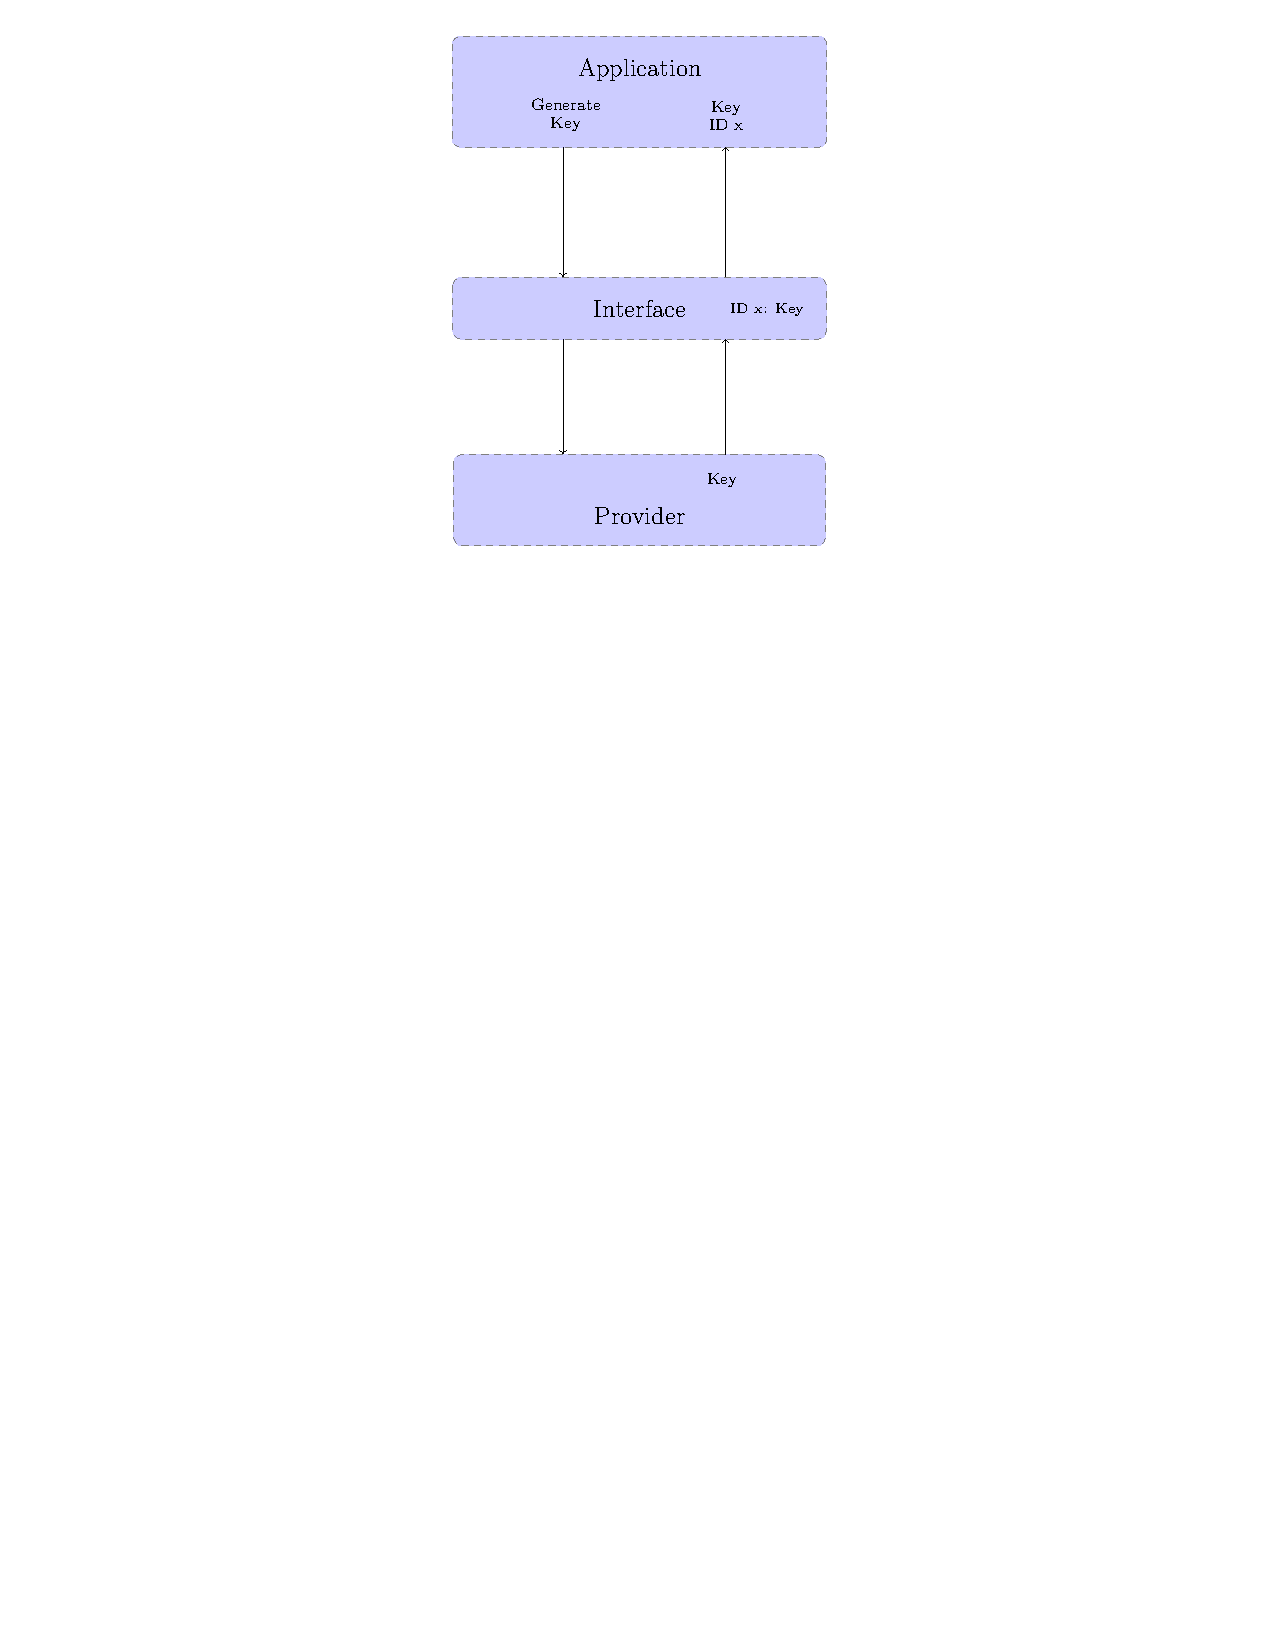
\includegraphics[trim=7cm 18cm 12cm 0cm,
height=6.5cm]{figures/interface_key_manag_gen_key.pdf}
%}
}


\only<2>{
%\frame{
% trim: left, bottom, right, up
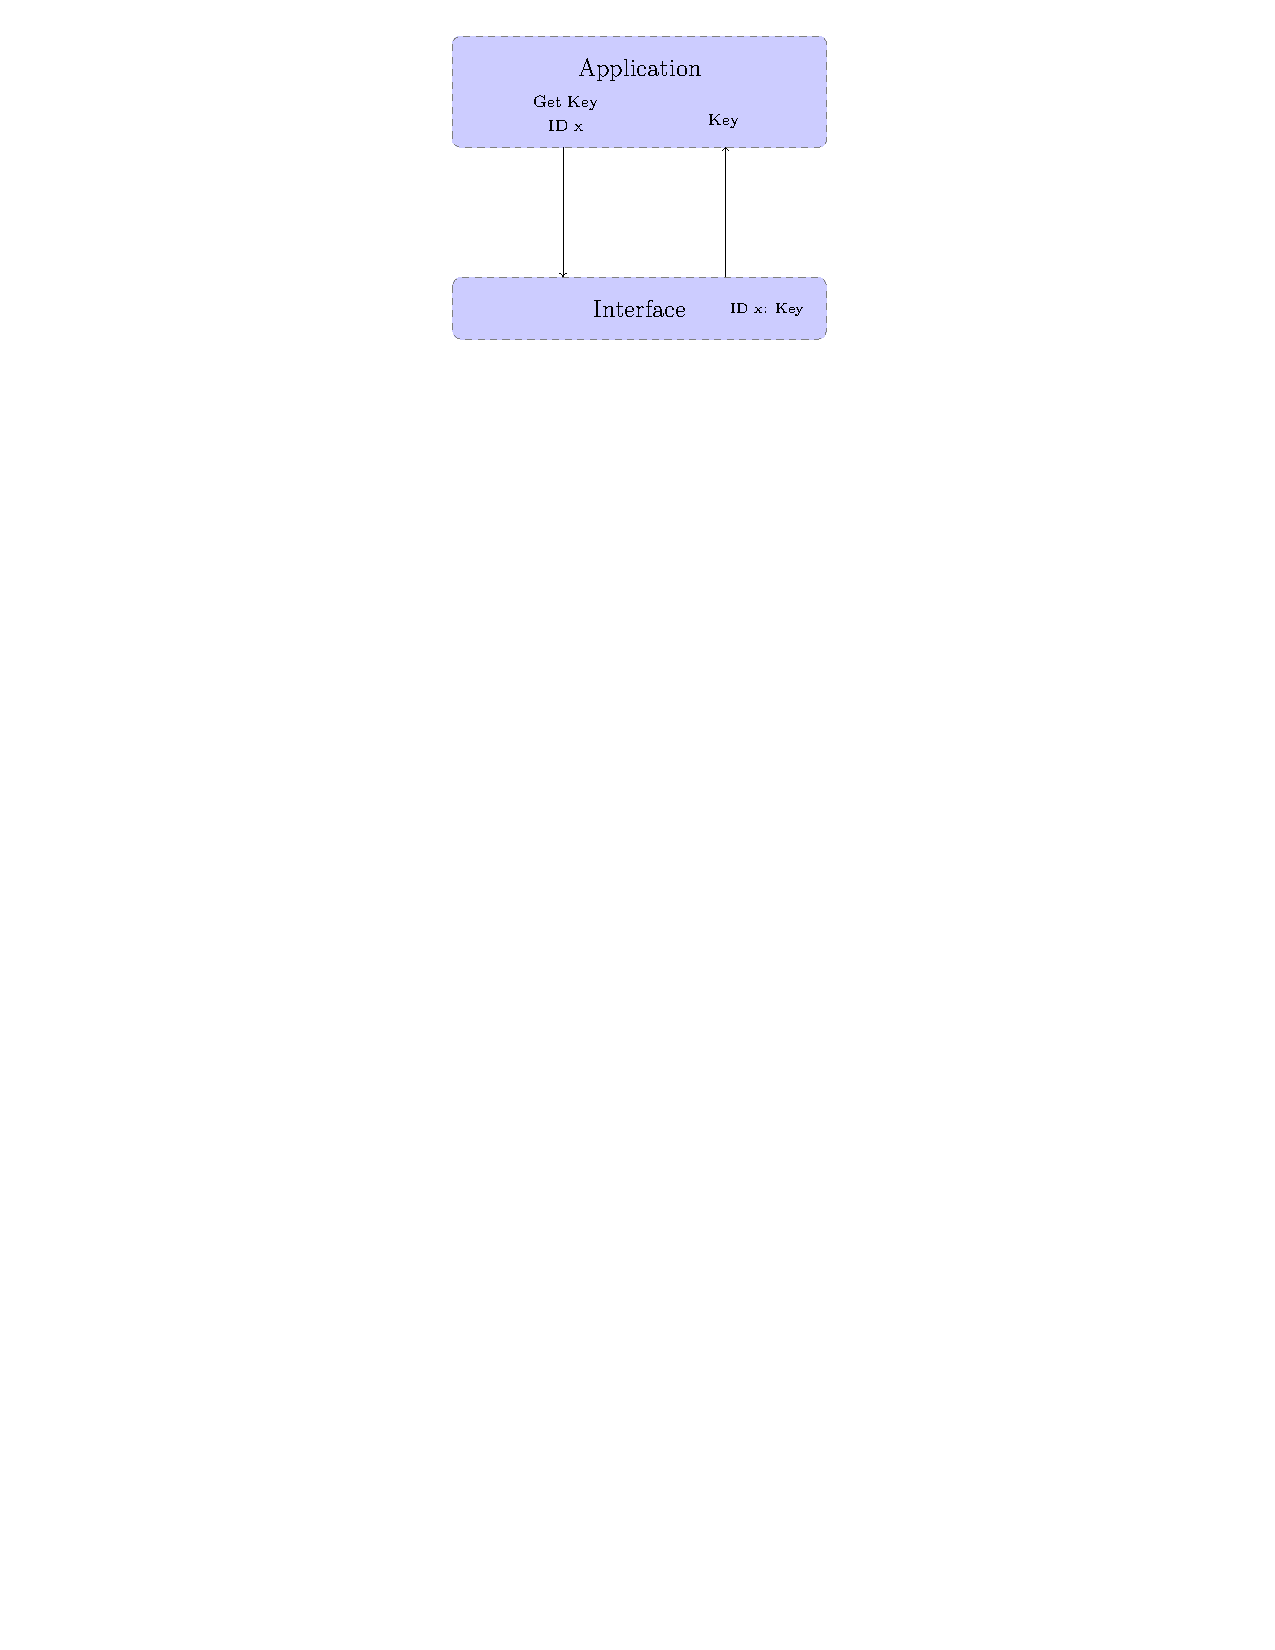
\includegraphics[trim=7cm 18cm 12cm 0cm,
height=6.5cm]{figures/interface_key_manag_get_key.pdf}
%}
}


\only<3>{
%\frame{
% trim: left, bottom, right, up
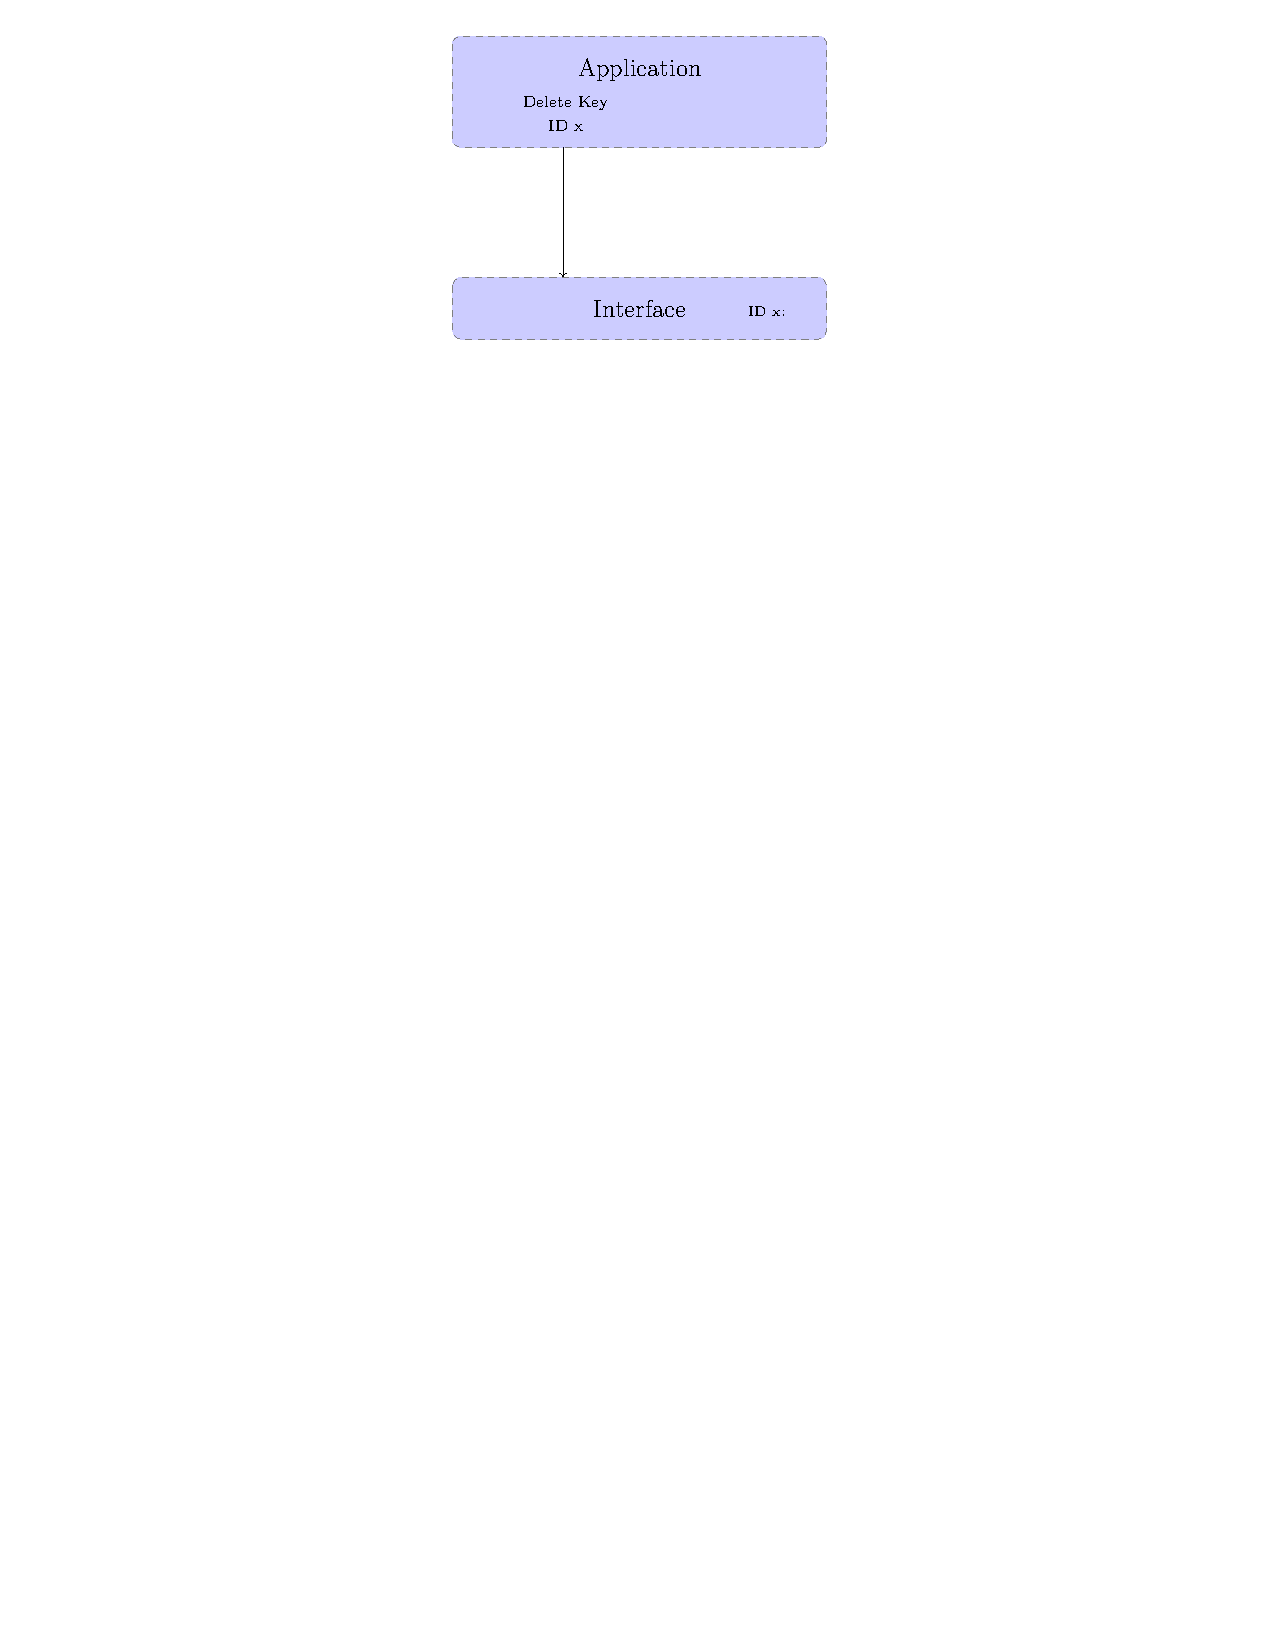
\includegraphics[trim=7cm 18cm 12cm 0cm,
height=6.5cm]{figures/interface_key_manag_del_key.pdf}
%}
}


\only<4>{
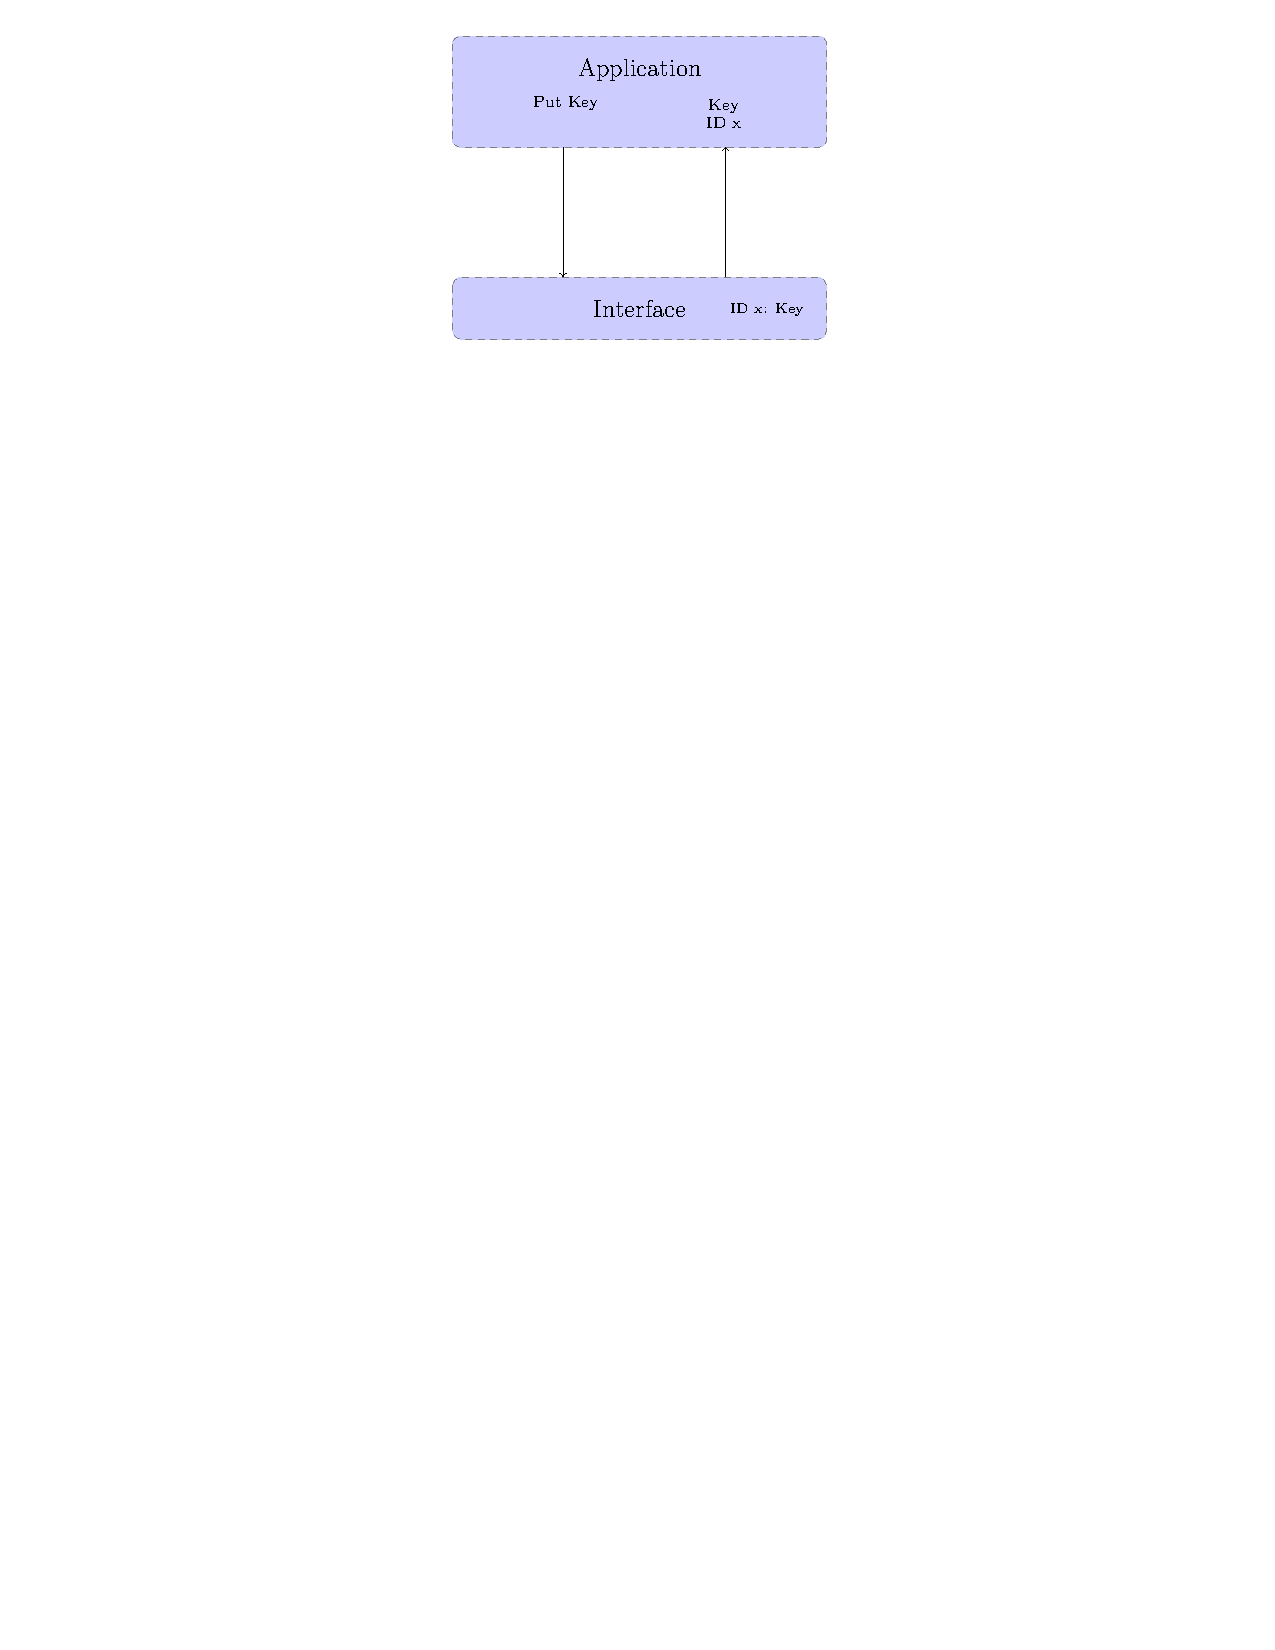
\includegraphics[trim=7cm 18cm 12cm 0cm,
height=6.5cm]{figures/interface_key_manag_put_key.pdf}

}

\end{column}

\begin{column}{0.6\textwidth}
\begin{itemize}
  \item Interface shall enable the use of a provider's internal key managemet services
\end{itemize}

\vspace{1cm}

\underline{Key management}:
\begin{itemize}
\only<1>{
  \item Generate the key and store it in the interface
  \item Return an ID which identify the key
}

\only<2>{
  \item Get the key by passing the ID
}

\only<3>{
  \item Delete the key by passing the ID
}

\only<4>{
  \item Store a key coming from outside (not generated by the
  provider) in the interface
  \item Return an ID which identify the key
}
\end{itemize}

\end{column}

\end{columns}



\end{frame}


\begin{frame}

\frametitle{Example: Cipher}


% trim: left, bottom, right, up
\centering
{
\only<1>{

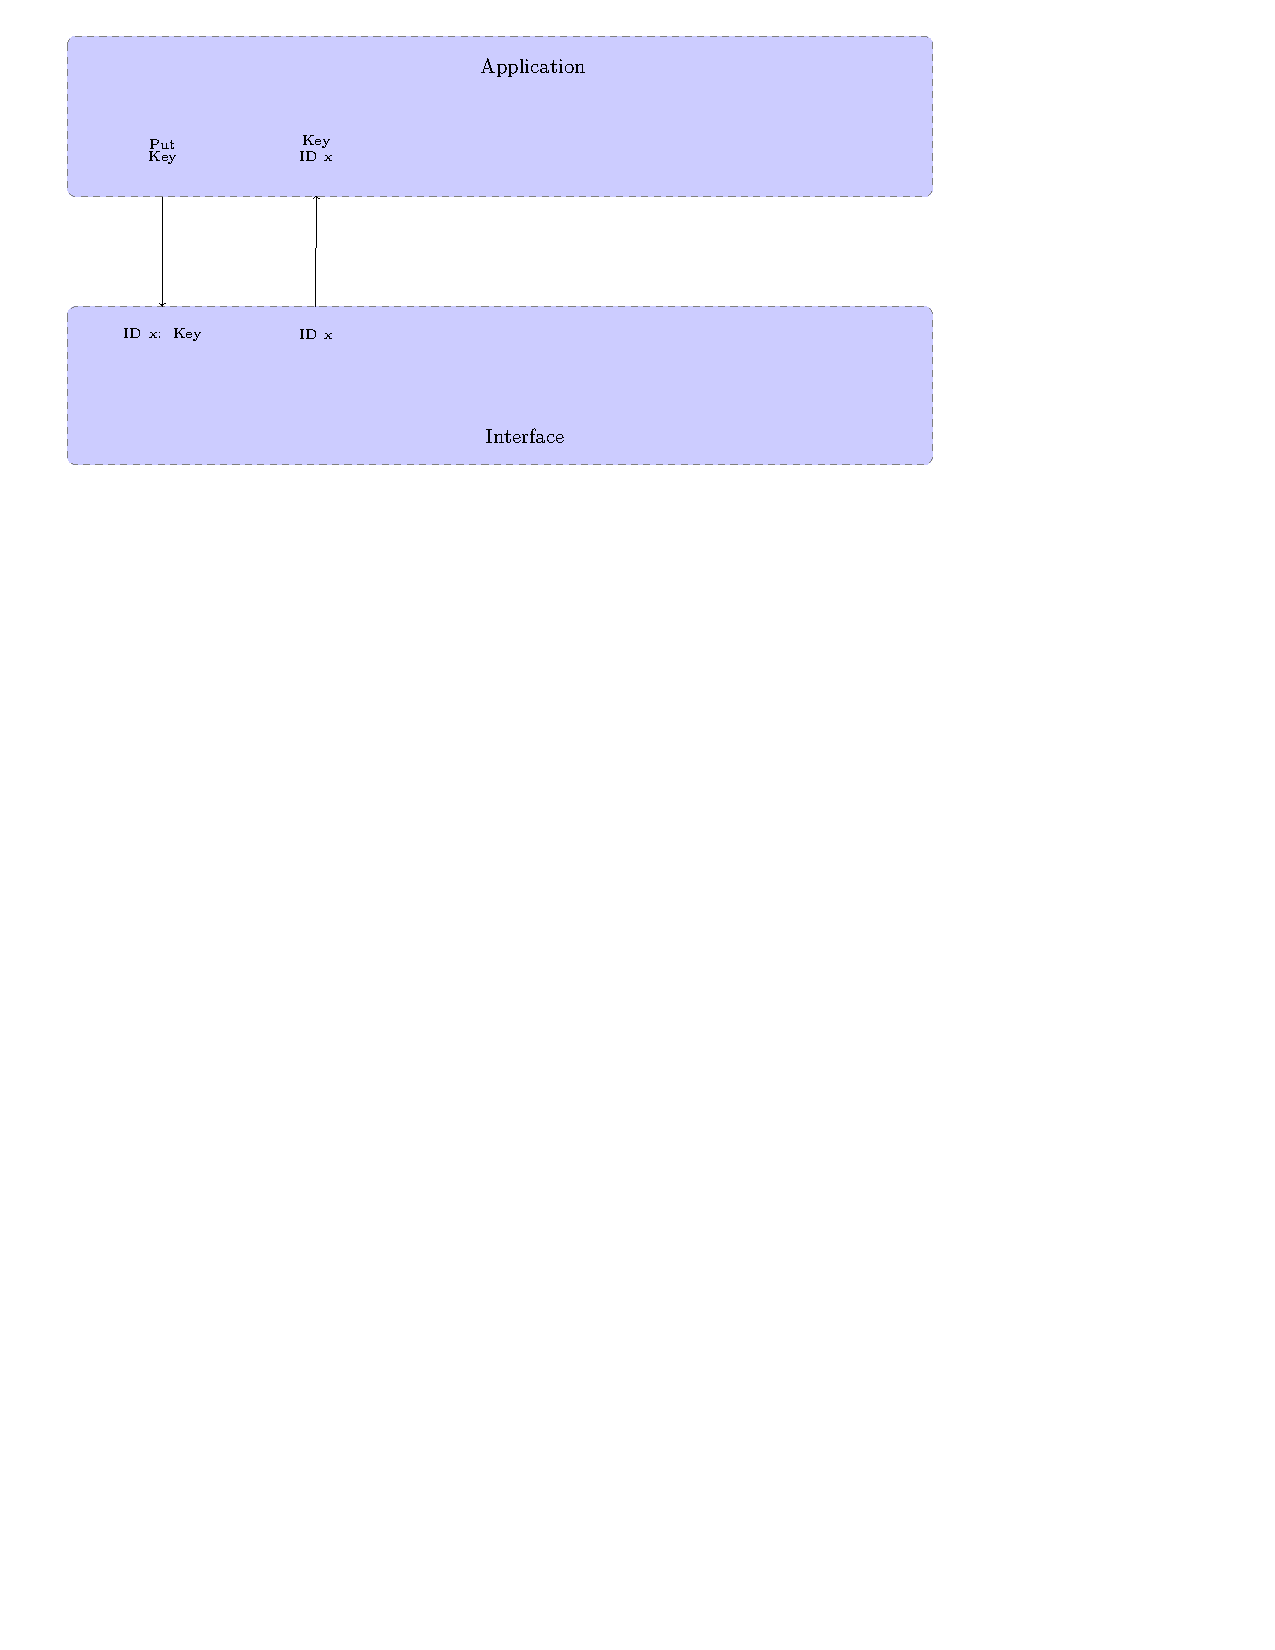
\includegraphics[trim=2cm 20cm 7cm 0cm,
height=5cm]{figures/interface_cipher_example_put_key.pdf} 

}


\only<2>{

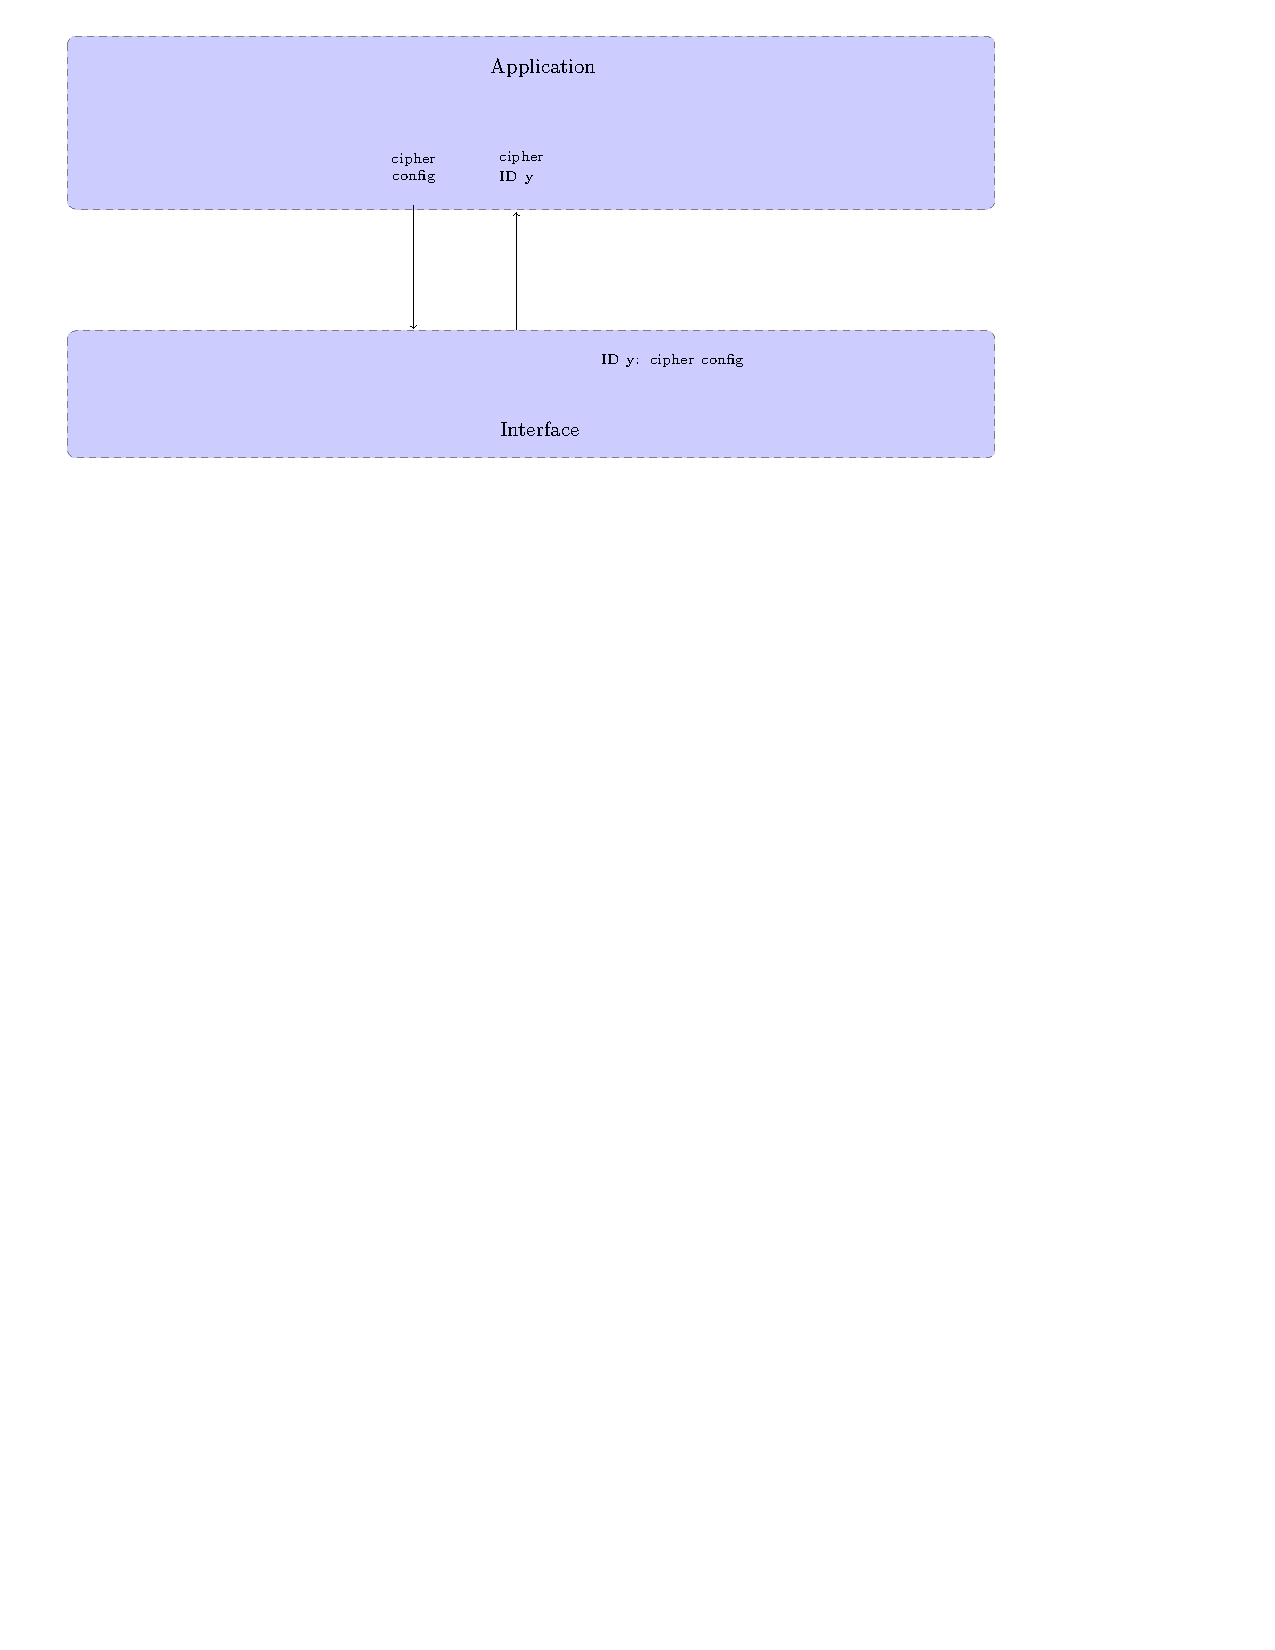
\includegraphics[trim=2cm 20cm 7cm 0cm,
height=5cm]{figures/interface_cipher_example_config.pdf} 

}


\only<3>{

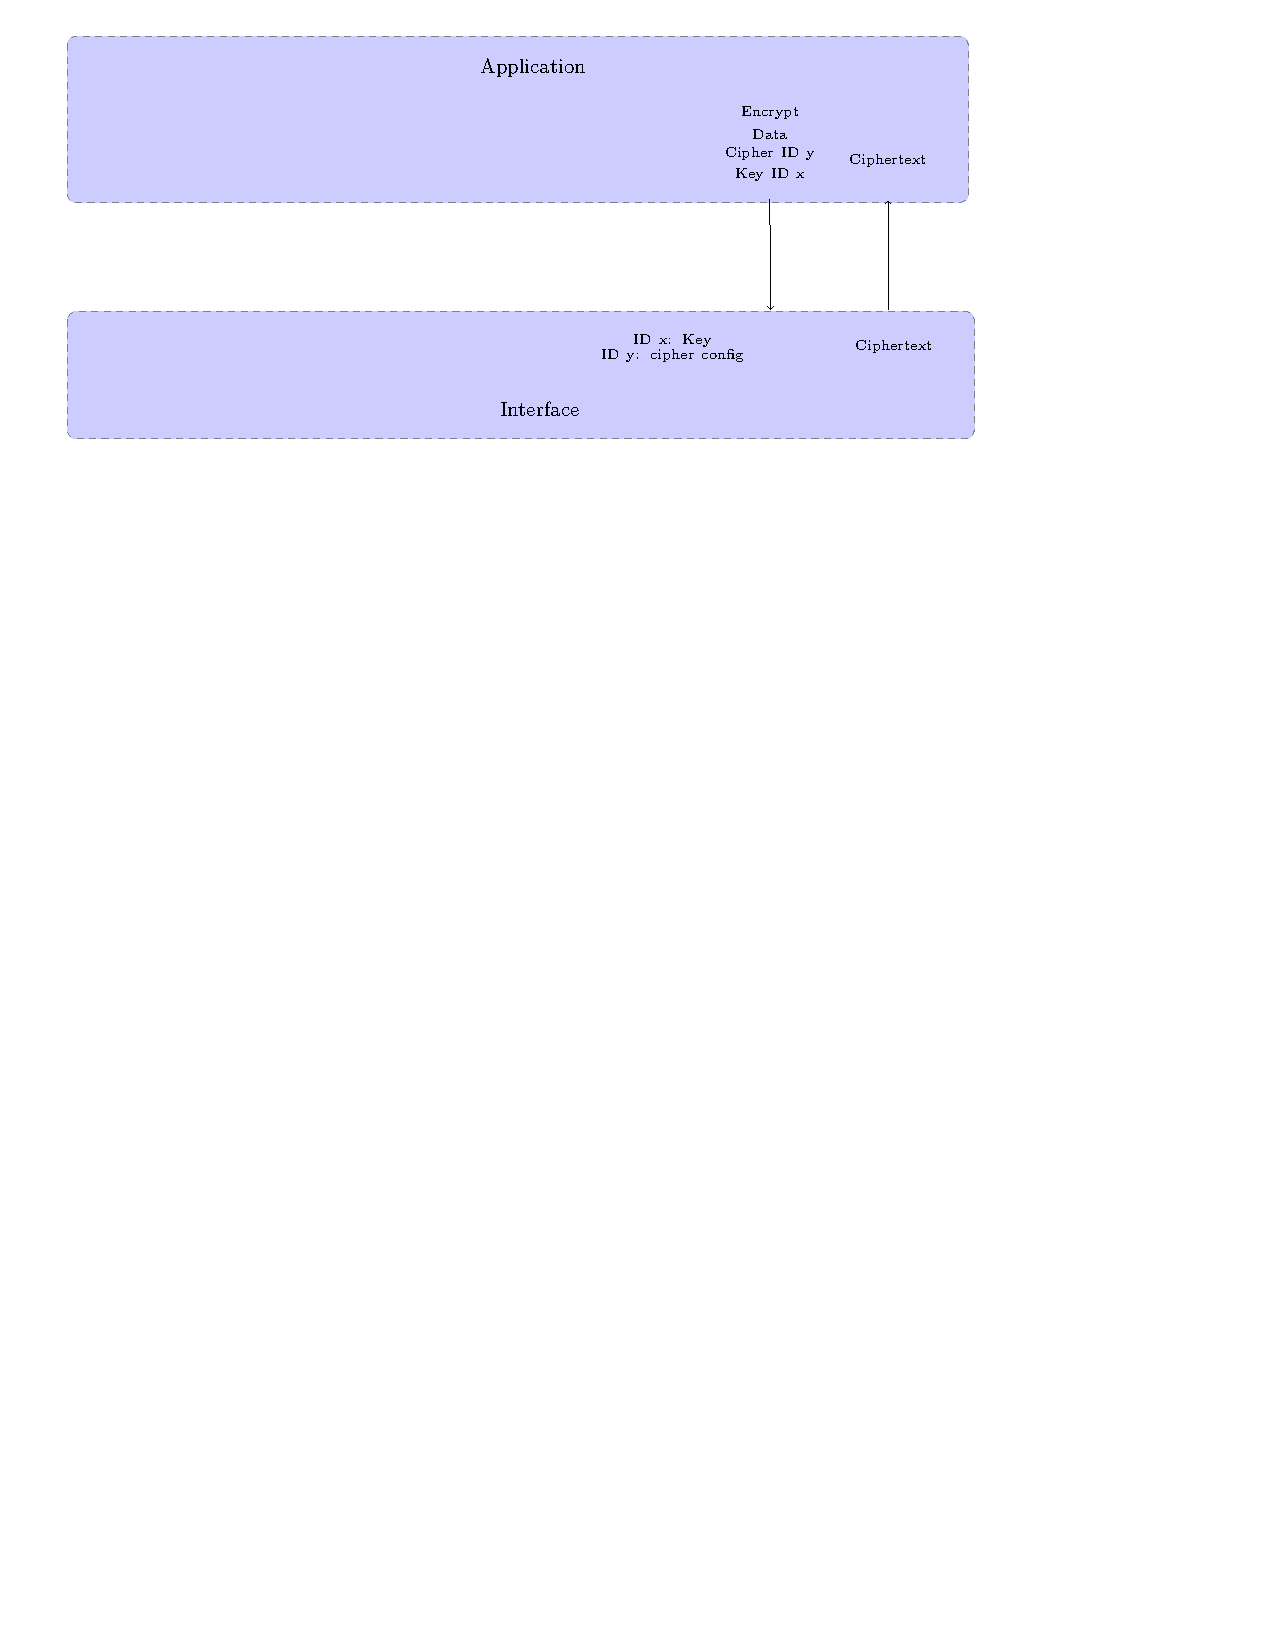
\includegraphics[trim=2cm 20cm 7cm 0cm,
height=5cm]{figures/interface_cipher_example_finish.pdf} 

}

}


\begin{enumerate}
  \item \footnotesize{Put a key coming from outside to the interface}
  \pause
  \item \footnotesize{Create the cipher context with the desired configuration}
  \pause
  \item \footnotesize{Encrypt a data with the key and configuration done
  previously}
\end{enumerate}

\end{frame}
